\chapter{Appendix}

\section{Learning from other sources of data}
\label{sec:search_engine_details}
% \begin{figure}[t!]
%     \centering
%     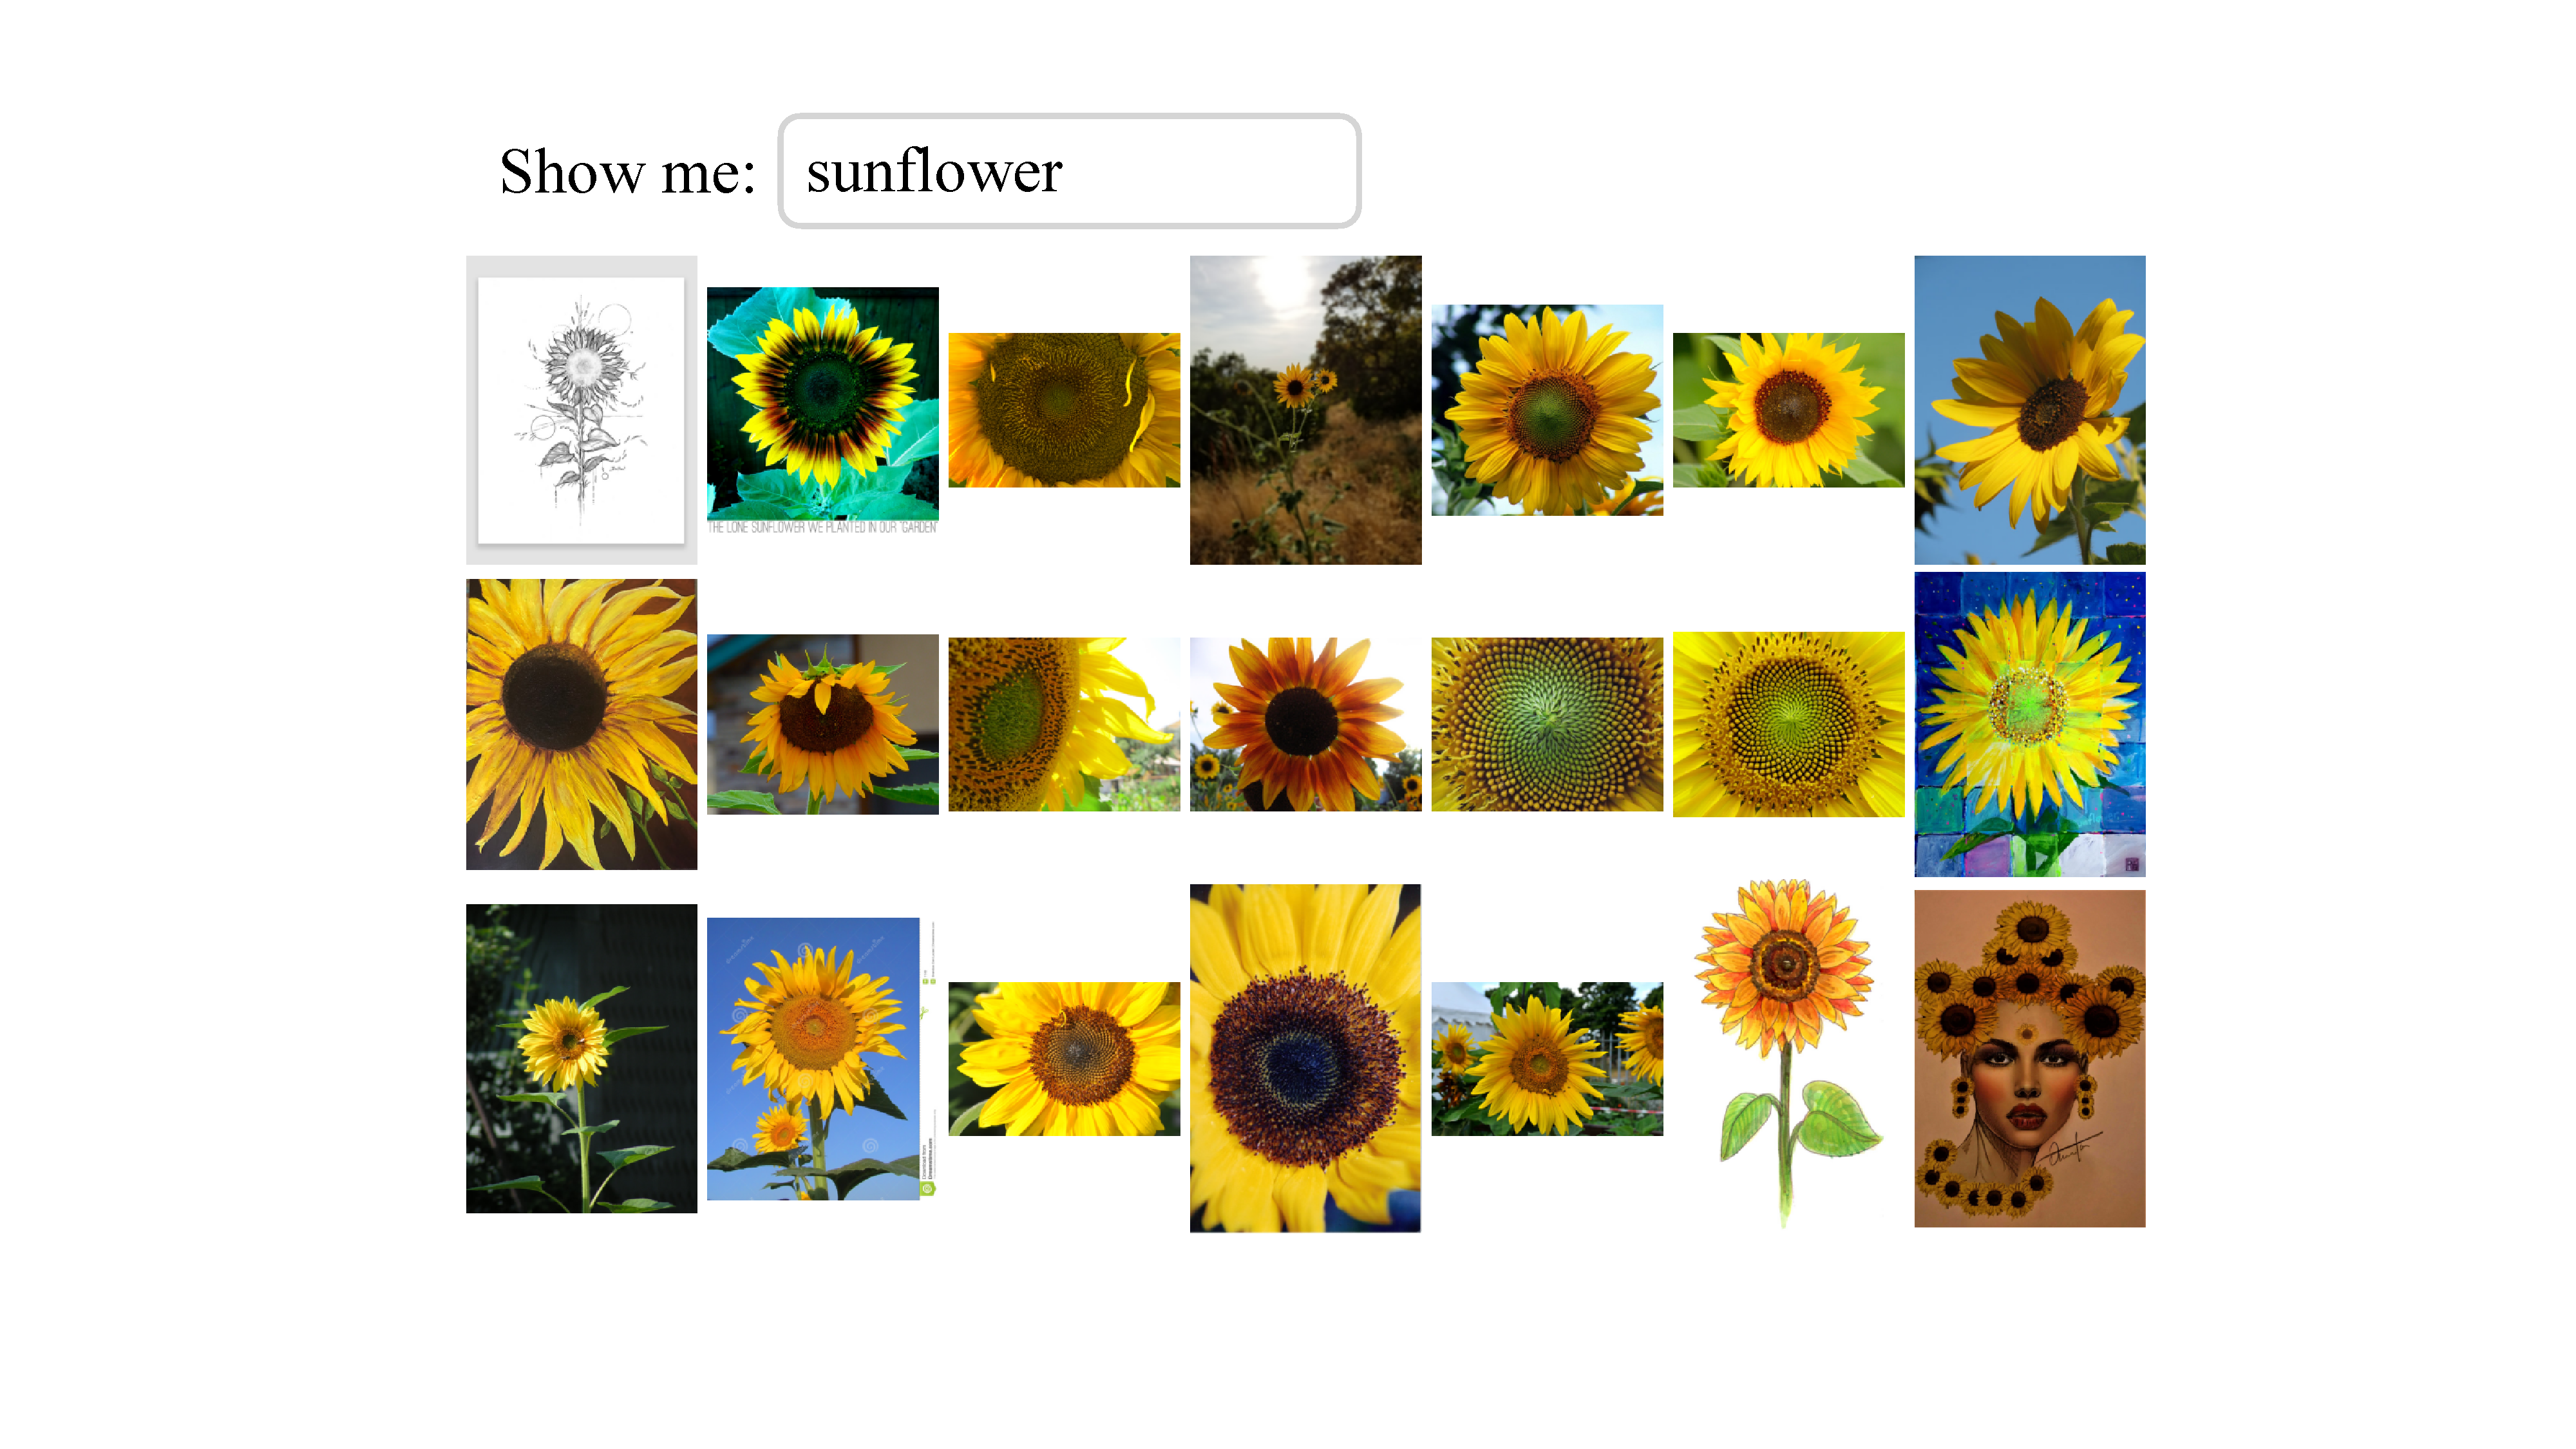
\includegraphics[width=0.4\linewidth]{figures/laion_search_engine.pdf}
%     \vspace{-1em}
%     \label{fig:laion_search_engine}
% \end{figure}
\begin{wrapfigure}{R}{0.4\textwidth}
\centering
    \vspace{-1.5em}
    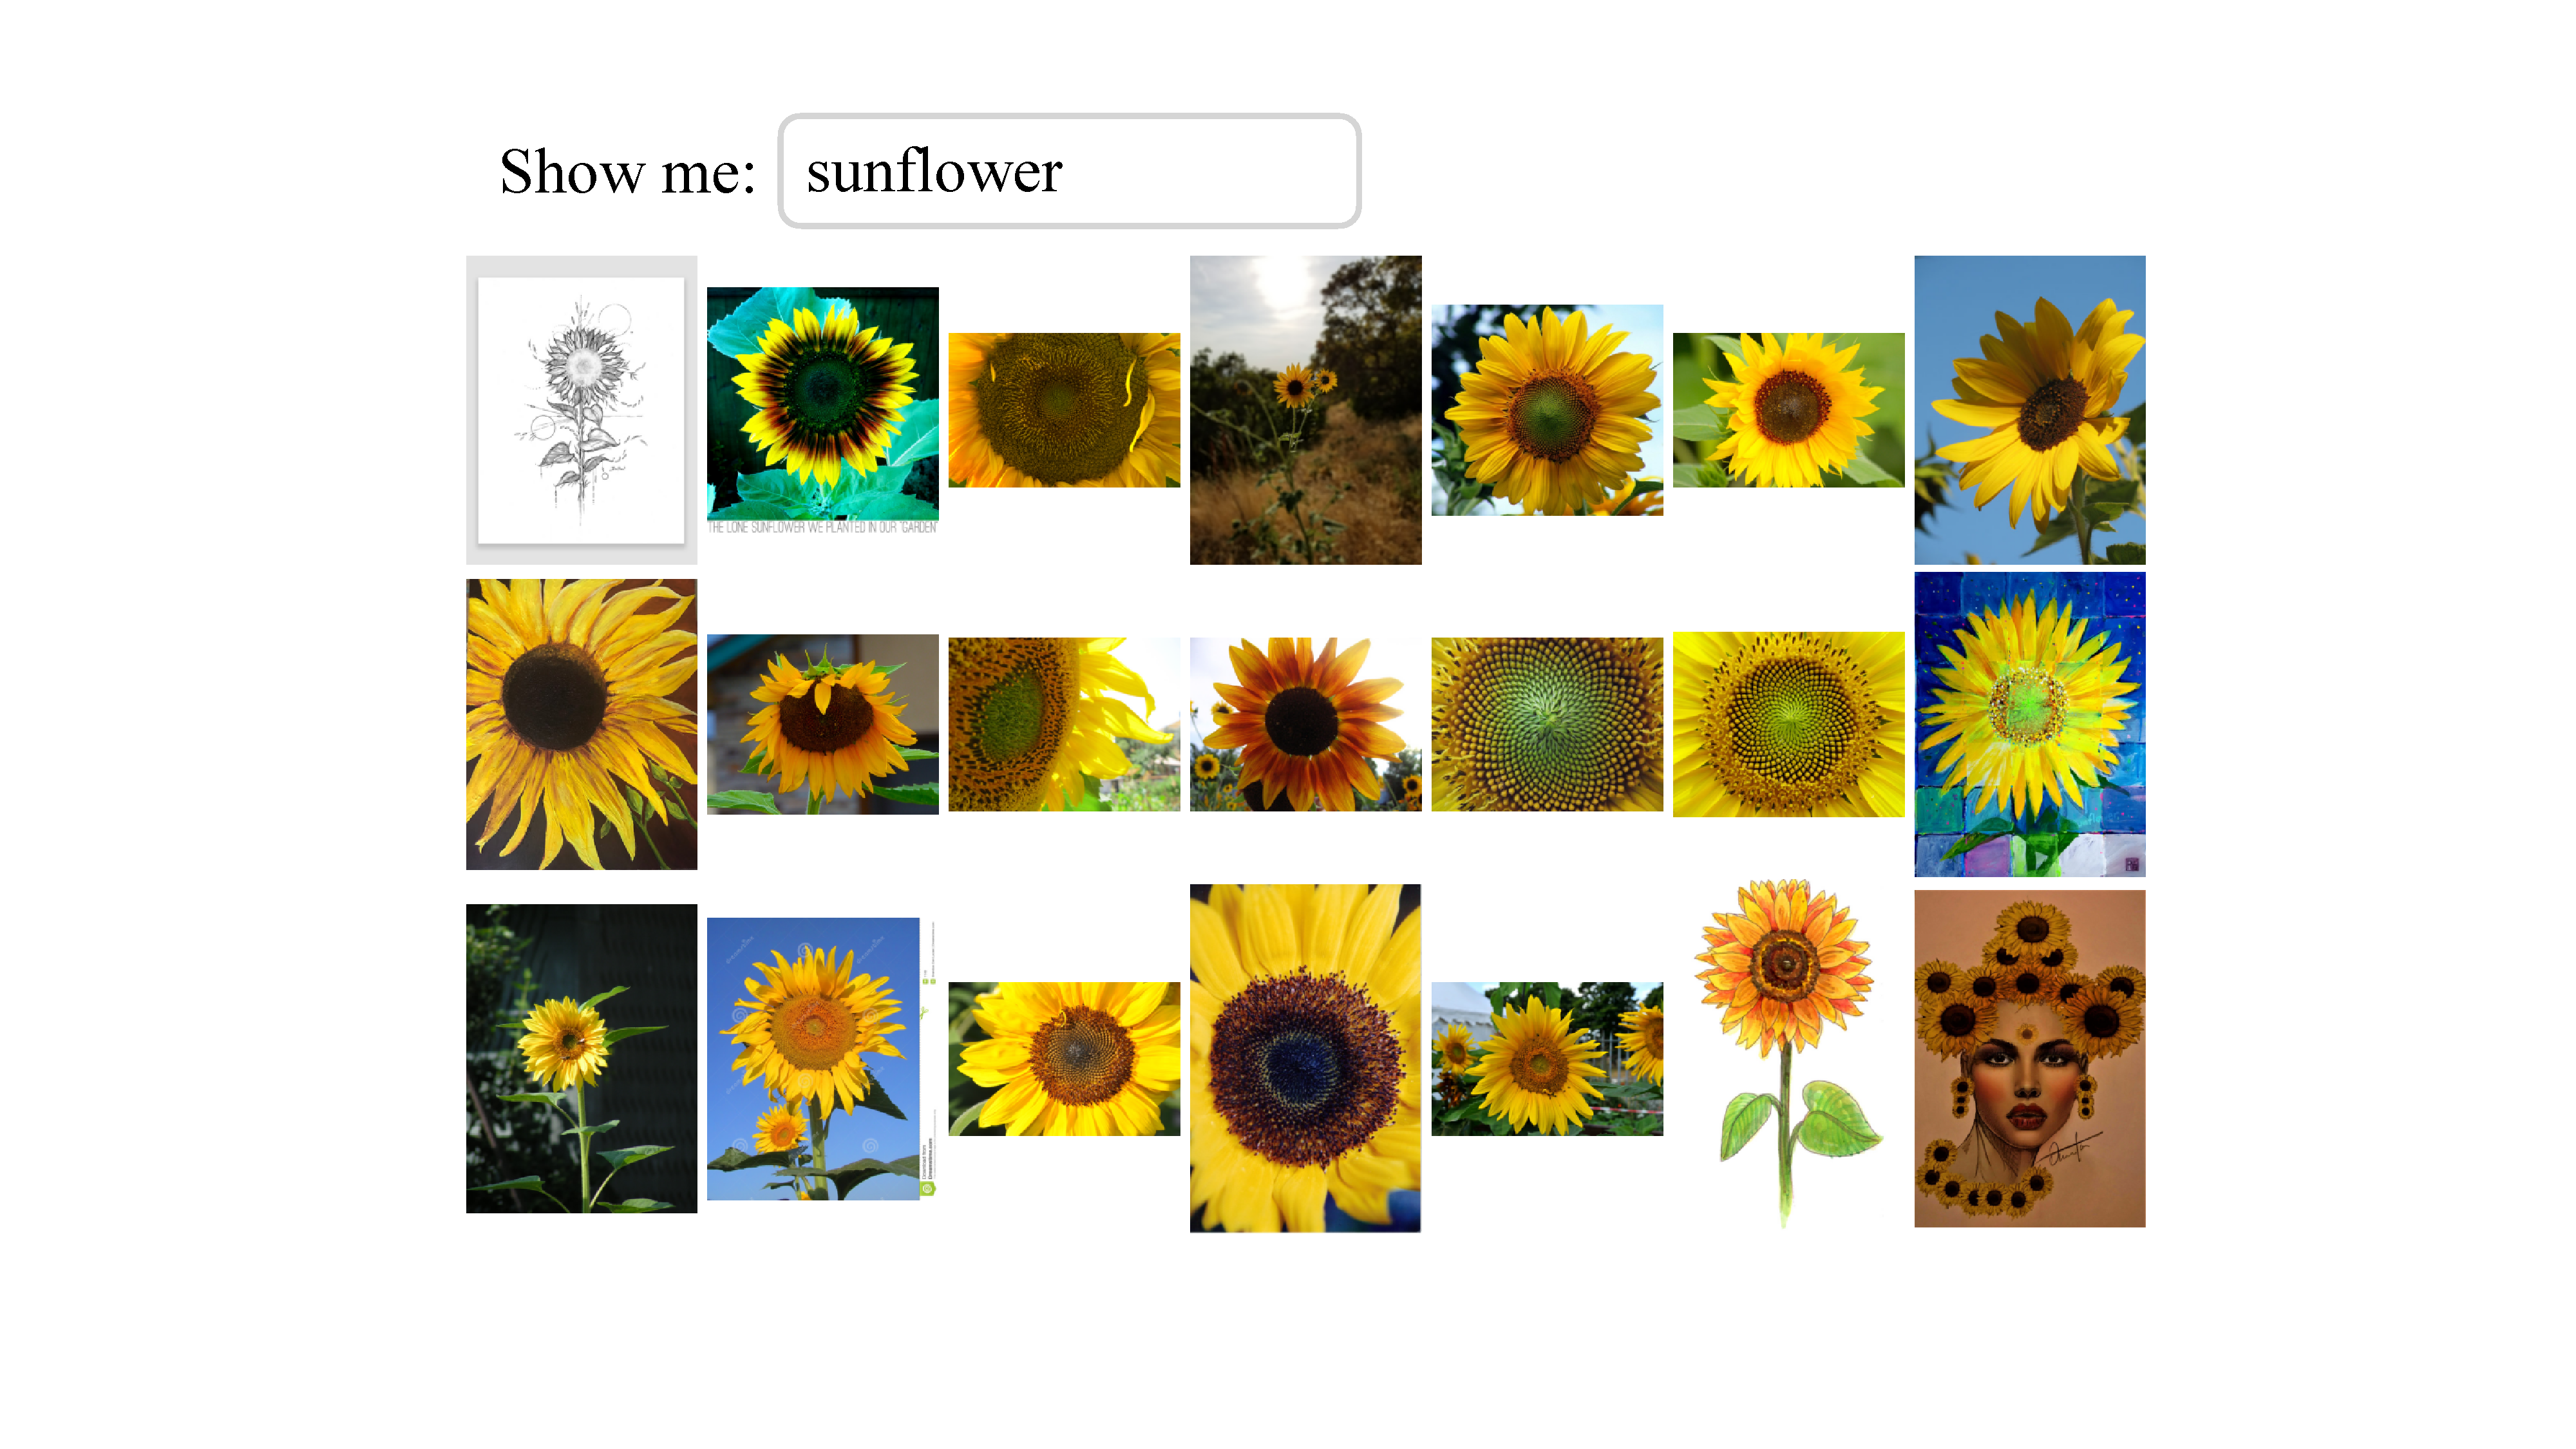
\includegraphics[width=\linewidth]{figures/laion_search_engine.pdf}
    \vspace{-1em}
    \caption{\textbf{Our custom LAION-5B search engine.} We build a custom text-to-image search engine that finds images within the LAION-5B dataset by doing nearest neighbor search in text embedding space. This uses no image features whatsoever.}
    \label{fig:laion_search_engine}
\end{wrapfigure}

Google Images is an exceptionally useful data source for Internet Explorer. It offers access to a large portion of the Internet's images, and it ranks images using weak supervision from the image caption, surrounding text, click rates, image features, incoming and outgoing hyperlinks, and other signals. This extra supervision is helpful and should be utilized. Nonetheless, we show that Internet Explorer is agnostic to the choice of text-to-image search engine and can still rapidly improve even when the data source is much noisier. 

To test Internet Explorer in the most minimal setting, we build a custom search engine that finds images solely using their accompanying text, without using any pre-trained visual features whatsoever. We use the LAION-5B dataset~\cite{schuhmann2022laion}, which consists of 5.85 billion noisy image-caption pairs. We filter the dataset to only include samples with English captions and images with at least $512^2$ pixels. This leaves us with about 600M text-image pairs. To find image results for a query, we find the 100 captions closest to the query in text representation space, then return the associated images.
We use a pre-trained text embedding model~\cite{reimers2019sentence} to compute 384-dimensional text embeddings for each caption. Then, we use Faiss~\cite{johnson2019billion} to compute a fast, approximate nearest-neighbors lookup index. Querying our custom search engine finds 100 image results in less than a second. \cref{fig:laion_search_engine} shows that our search engine is reasonably accurate, even without using any image features. 

We also test Flickr's photo search API as another text-to-image search engine, in addition to Google Images and LAION. \cref{fig:data_comparison} shows that each data source has its own tendencies. For the ``spaghetti bolognese'' query, Google Images is biased~\cite{mezuman2012learning,chen2015webly} towards brightly-lit, photogenic images that typically come from food blogs. Flickr mainly consists of amateur home photos, so it returns a messier variety of images that perhaps better capture the real world. LAION images come from web crawling, without any ranking, so they additionally contain many graphics with text overlays. The same image can also frequently show up in the LAION results multiple times, as a result of being posted on multiple separate pages. 


\begin{figure*}
    \centering
    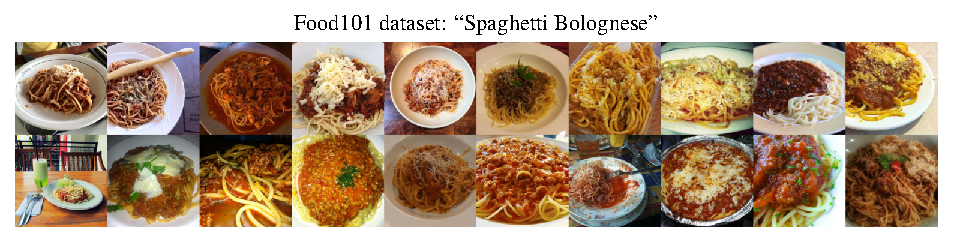
\includegraphics{figures/food-spaghetti.pdf} \\
    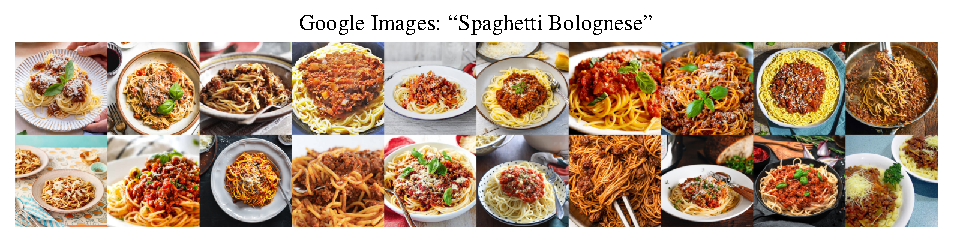
\includegraphics{figures/google-spaghetti.pdf} \\
    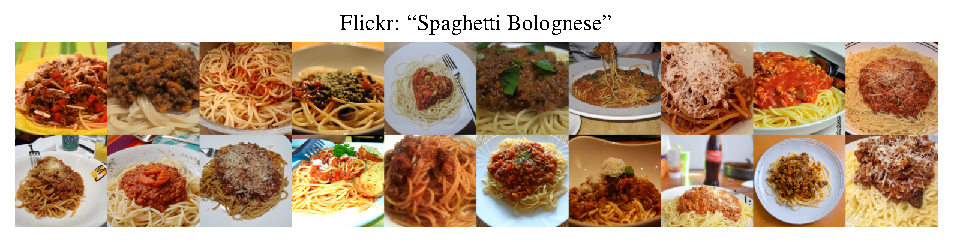
\includegraphics{figures/flickr-spaghetti.pdf} \\
    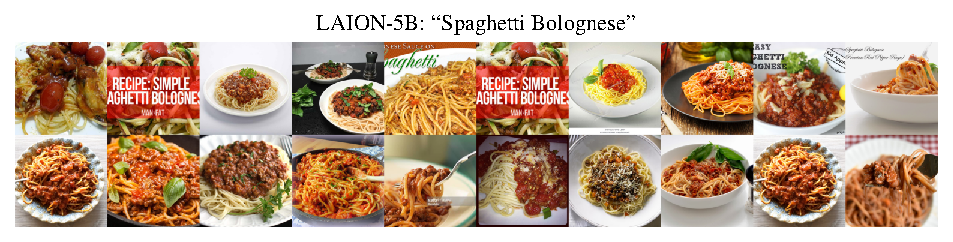
\includegraphics{figures/laion5b-spaghetti.pdf} 
    \caption{\textbf{Comparison of different search engines.} We show images for the ``spaghetti bolognese'' class in the Food101 dataset, as well as 20 search results for ``spaghetti bolognese'' from Google Images, Flickr, and LAION5B. Google images are typically well-lit, aesthetic food blog pictures. In comparison, Flickr images are messier, darker, and capture a wider variety of real-world conditions. LAION-5B images lie somewhere in the middle, but contain text overlays much more frequently. Duplicate image results are also common.}
    \label{fig:data_comparison}
\end{figure*}

\begin{figure*}
    \centering
    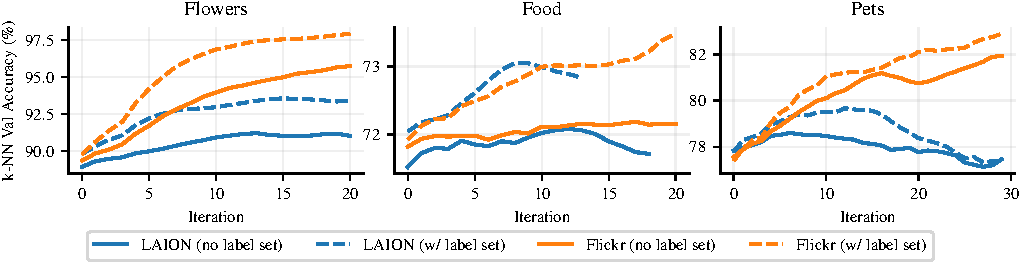
\includegraphics{figures/laion-curves.pdf}
    \caption{\textbf{Learning from Flickr and LAION-5B.} Even with the noisy search results returned by Flickr and LAION, Internet Explorer still continuously improves performance. }
    \label{fig:other_data_curves}
\end{figure*}


% We use Internet Explorer to efficiently search our new data sources: LAION-5B and Flickr. 
\cref{fig:other_data_curves} and \cref{tab:search_engine} show that Internet Explorer still improves over time, even when the data comes from LAION or Flickr. 
Internet Explorer tends to perform better with Flickr than with LAION, which makes sense. Flickr indexes far more images, as our custom LAION search engine only uses 600M images, so it can return more of the useful photos that Internet Explorer queries for. Flickr is also slightly better at understanding descriptors, although both Flickr and LAION tend to be thrown off by specific or odd descriptors. Nevertheless, even with noisy search results and no hyperparameter tuning, Internet Explorer significantly improves the starting model in less than a day of searching and training. Overall, these results are a proof of concept that Internet Explorer can effectively utilize any window into the Internet's vast ocean of image data. 


\section{Are we finding the entire test set online?}
\label{sec:finding_test_set_online}
\begin{table*}[t]
    \centering
    \begin{tabular}{lccccccccc}
    \toprule
        % Model & Flowers102 & Food101 & Stanford Cars & Oxford-IIIT Pets & Total Images & GPU-hours \\
        Model & Birdsnap & Flowers & Food  & Pets & VOC2007  & Images Downloaded \\
    \midrule
    \textit{No exploration} \\
        \;\;\; Target training set                          &  $1/1849$ &  $5/6142$ & $34/25246$ & $21/3663$ &  $0/4952$ & $-$ \\
    \midrule
    % \textit{No label set information} \\
    \textit{Internet Explorer} \\
        % \;\;\;Random exploration                     &  ? &  ? &  ? &  ? &  ? \\
        % \;\;\;Ours                                   &  ? &  ? &  ? &  ? &  ? \\
        \;\;\;Ours++ (no label set)                         &  $28/1849$ & $11/6142$ & $35/25246$ & $26/3663$ & $1/4952$ & $\approx 10^6$\\
    % \midrule 
    % \textit{Use label set information} \\       
        % \;\;\;Search labels only                      &  ? &  ? &  ? &  ? &  ? \\
        % \;\;\;Labels + semantically relevant terms    &  ? &  ? &  ? &  ? &  ? \\
        % \;\;\;Ours                                    &  ? &  ? &  ? &  ? &  ? \\
        \;\;\;Ours++ (with label set)                       & $57/1849$ & $27/6142$ & $35/25246$ & $43/3663$ & $1/4952$ & $\approx 10^6$ \\
    \bottomrule
    \end{tabular}
    \caption{\textbf{Number of leaked test set images}. We use image hashing to compute the fraction of test images present in the set of images downloaded by Internet Explorer.  We show (number of leaked images)$/$(number of unique test images). Surprisingly, the training sets of these datasets already leak a small fraction of the test sets. Leakage numbers for our methods include this train-test leakage, since our methods use the target dataset's training set. Internet Explorer only finds a tiny fraction of test set images online, and it only uses them for self-supervised training, so there is no \textit{label leakage}. Overall, Internet Explorer's increase in accuracy cannot be explained by test set leakage, so it must be improving performance through better feature learning and generalization.
    }
    \label{tab:leakage}
\end{table*}
One may be concerned that Internet Explorer improves performance mainly by finding a significant portion of the test set images online. We address this concern by checking how much test data Internet Explorer has downloaded. We use difference hashing (dHash)~\cite{imagehash} to compute hashes for the target dataset's training set, its test set, and the downloaded Internet data. We compare hashes to determine how many test images were leaked, and we report the number of collisions in \cref{tab:leakage}. Across all five datasets, Internet Explorer finds very few test images. On Birdsnap, Internet Explorer finds 56 additional test set images that were not leaked in the training set, which is roughly $3\%$ of the test set. On the other datasets, the amount leaked ranges from $0.003\%$ to $0.6\%$ of the test set. Additionally, we only perform self-supervised training on downloaded images, so it is much harder for our model to cheat with the leaked images. Overall, given that Internet Explorer outperforms its starting checkpoint by between 5 to 30 percentage points, we conclude that its performance cannot be explained by cheating. 

\section{Method Details}

% We draw our concepts from the WordNet hierarchy~\cite{miller1995wordnet}, which consists of $146{,}347$ noun lemmas. Not all of these lemmas are visual, but the vocabulary still covers an incredible range of topics.
% % For reference, here are 6 randomly sampled concepts:  {\tt {\small `sleep talking', 
% % `beach wagon', `Balearic Islands', `borosilicate', `genus Loranthus', `humpback whale'}}.
% We can generate descriptors for each concept by prompting a GPT-J language model~\cite{gpt-j} with examples of descriptor-concept pairs (details in the supplementary).
% % For reference, here are 7 randomly sampled descriptors for ``labrador retriever'': {\tt {\small `friendly', `short', `long-legged', `big', `fast', `blue-eyed', `handsome'}}.

\subsection{WordNet Lemmas}
\label{sec:wordnet_lemmas}
We draw our concepts from the WordNet hierarchy~\cite{miller1995wordnet}, which consists of $146{,}347$ noun lemmas. For reference, here are 32 randomly sampled concepts:
\begin{quote}
{\tt { 
% `sleep talking', `beach wagon', `Balearic Islands', `borosilicate', `genus Loranthus', `humpback whale'
"resolution",
"lodgment",
"phycobilin",
"acidosis",
"widening",
"human face",
"family Crassulaceae",
"sail",
"Ipomoea imperialis",
"Davis",
"prothrombin",
"cease",
"marsh clematis",
"major power",
"chump change",
"madcap",
"junky",
"pere david's deer",
"make-up",
"genus Rumex",
"gape",
"Brachychiton populneus",
"bell morel",
"wain",
"friendly",
"Principe",
"bottle green",
"glycerol trimargarate",
"water-shield",
"San Joaquin River",
"woodsman",
"pin".
}}
\end{quote}

\subsection{GPT-J Descriptor Prompting}
\label{sec:gptj-descriptors}
We use GPT-J-6B~\cite{gpt-j}, a free, open-source autoregressive language model, to generate useful descriptors for a given concept. We use the following prompt template: 
\begin{itemize}
    \item[] \texttt{"What are some words that describe the quality of `\{concept\}'?} 
    \item[] \texttt{The \{concept\} is frail.}
    \item[] \texttt{The \{concept\} is red.}
    \item[] \texttt{The \{concept\} is humongous.}
    \item[] \texttt{The \{concept\} is tall.}
    \item[] \texttt{The \{concept\} is"}
\end{itemize}

We sample completions with a temperature of 0.9 and a max length of 100 tokens. We truncate the completion after the first comma, period, underscore, or newline character (including the special character). If the truncated completion is degenerate and contains a duplicate of the concept, we resample another completion. After successfully sampling a descriptor, we prepend it to the concept and use the resulting phrase as our search query. 

% - TODO: put in a page of examples.   
% - Pencil: 'fragile', 'huge!', 'too big', 'colorful', 'dark', 'too soft', 'blunt', 'narrow', 'round', 
% 'blue', 'black', 'a soft piece of wood', 'thick', 'heavy', 'light', 'short'
% - TODO: These descriptors generally 
% - Our prompt can be easily 

For reference, here are 32 randomly sampled descriptors for ``labrador retriever'':
% {\tt {\small `friendly', `short', `long-legged', `big', `fast', `blue-eyed', `handsome'}}.
\begin{quote}
{\tt { 
% `sleep talking', `beach wagon', `Balearic Islands', `borosilicate', `genus Loranthus', `humpback whale'
"a good-looking dog",
"very gentle",
"a",
"brown",
"lovable",
"a strong runner",
"a male or a female",
"sturdy",
"agile",
"a strong",
"beautiful",
"a male",
"kind",
"long-haired",
"a male or a female",
"a good-looking dog",
"gentle",
"medium",
"loyal",
"very gentle",
"blue-eyed",
"sturdy",
"blue-eyed",
"a retriever",
"kind",
"loyal",
"large",
"brown",
"good-natured",
"gentle",
"large",
"small".
}}
\end{quote}



\subsection{Concept Vocabulary Size}
\label{sec:concept_vocab_size}
As stated in Section \ref{subsec:text_query_generation}, our vocabulary comprises the $146{,}347$ noun lemmas in the WordNet hierarchy. Thus, in all our experiments, Internet Explorer only searches for WordNet terms (plus the class names, if we have knowledge of the label set). We found that this worked quite well for these standard benchmarks. Note that expanding the vocabulary (e.g., adding technical terms relevant to a specific topic) can easily be done by adding those terms to the list of possible concepts. One easy extension would be to add page titles and frequent unigrams and bigrams from Wikipedia, as was done to generate the CLIP training set~\cite{radford2021learning}. Doing so would expand our vocabulary to roughly $500{,}000$ total concepts. 

\subsection{Query Model Details}
\label{sec:query_model_details}
\paragraph{Temperature for concept distribution}
After estimating scores $r(c_i)$ for each concept $c_i$, we do a temperature-scaled softmax, followed by the tiering operation described in Section 2.6. We compute the temperature $\tau$ such that 
\begin{align}
     \text{SMR} = \frac{\max_i r(c_i) - \min_i r(c_i)}{\tau}
\end{align}
where the ``softmax range'' $\text{SMR} \in \mathbb R$ is the desired gap between the largest and smallest scores after temperature scaling. After the softmax $p(c_i) \propto \exp(r(c_i) / \tau)$, the softmax range determines the likelihood ratio of most likely concept to least likely concept: 
\begin{align}
    \frac{\max_i p(c_i)}{\min_i p(c_i)} &= \frac{\max_i \exp(r(c_i) / \tau)}{\min_i \exp(r(c_i) / \tau)} \\
      &= \exp \left(\frac{\max_i r(c_i) - \min_i r(c_i)}{\tau}\right) \\
    &= \exp(\text{SMR})
\end{align}
Thus, SMR is an easy way to specify the relative likelihood of the highest and lowest scoring concepts and achieve a desired exploration-exploitation balance. 


\paragraph{Label set-guided vocabulary}
% When we know the label set, 
% TODO(Ellis) describe the vocab subset creation for each dataset 
To reduce our search space in the label set-guided setting, in which we know the English names of the classes a priori, we generate a subset of the WordNet vocabulary that contains only the top-$10\%$ most semantically-relevant concepts to each target dataset.
We use a pre-trained text embedding model~\cite{reimers2019sentence} to generate $384$-dimensional embeddings for each concept in WordNet, using the same template described in Section 2.5 of the main paper: %, and reproduced below:

\begin{quote}
\vspace{-0.07in}
{\tt {\small \{lemma\} (\{hypernym\}): \{definition\}}}.
\vspace{-0.07in}
\end{quote}

To generate a similar embedding for concepts in target datasets, we use the summary from Wikipedia in place of the definition and the ``category'' of the target dataset (shown in \cref{tab:dataset_categories}) in place of the hypernym:

\begin{quote}
\vspace{-0.07in}
{\tt {\small \{label\} (\{category\}): \{summary\}}}.
\vspace{-0.07in}
\end{quote}


\begin{table}
    \centering
    \begin{tabular}{ll}
    \toprule
        Dataset & Category \\
    \midrule
        Oxford Flowers102 & Flower \\
        Oxford IIIT Pets & Pet \\
        Food101 & Food \\
        Birdsnap & Bird \\
        VOC2007 & Object \\
    \bottomrule
    \end{tabular}
    \caption{\textbf{Target Dataset ``Category''}.
    }
    \label{tab:dataset_categories}
\end{table}

After generating the embeddings for each concept in the target dataset, we find the $k$-NN distance for each WordNet concept to the target dataset embeddings, where $k$ is chosen to be $1/3$ the size of the class label set.
We then rank the concepts in WordNet by the distance and take the closest $10\%$ of terms as our subset. This subset is used for all methods in the label set-guided setting, including the random exploration methods. 






\subsection{Training Details}
In each iteration, we download roughly 25k candidate images, since we download up to 100 images for each of the 256 queries. Given this set $\mathcal C$ of candidate images, we sample $\text{PCR} \times |\mathcal C|$ images from the union of the replay buffer $\mathcal B$ and the target dataset training images $\mathcal D$. PCR (past data to candidate data ratio) is a scalar value that determines how much old data vs new data to train on at every iteration. We set $\text{PCR}=2$ for all experiments. We perform $10$ epochs of training over the union of the new candidate data and the sampled replay buffer and target dataset images. 

\subsection{Hyperparameters}
% privilege ratio, privilege gamma 
% k 
% GP 

\cref{tab:hyperparameters} shows our hyperparameter values, which are shared across datasets. We perform minimal hyperparameter tuning and copy most of the values from the MoCo-v3~\cite{chen2021empirical} ResNet-50 configuration. 
We will also release our code upon acceptance, which we hope will clarify any remaining implementation details and make it easy for the community to reproduce and build on our work. 
\begin{table}
    \centering
    % \begin{adjustbox}{width=\linewidth}
    \begin{tabular}{ll}
    \toprule
        Hyperparameter & Value \\
    \midrule
        Architecture & Resnet-50~\cite{he2016deep} \\
        Optimizer & LARS~\cite{you2017large} \\
        Batch size & $224$ \\
        Learning rate & $0.8 \times \frac{224}{256}$ \\
        Learning rate schedule & constant \\
        MoCo momentum & $0.9985$ \\
        RandomResizedCrop min crop area & $0.2$ \\
        % PCR & 2? \\
        Queries per iteration & $256$ \\
        Requested images per query & $100$ \\
        Min images per query & $10$ \\    
        Softmax range (SMR) & $3$ \\
        PCR & $2$ \\
        Epochs per iteration & $10$ \\
    \bottomrule
    \end{tabular}
    % \end{adjustbox}
    \caption{\textbf{Internet Explorer hyperparameters}.}
    \label{tab:hyperparameters}
\end{table}


\subsection{Image Licenses}
Internet Explorer uses images that were indexed by a web crawler (Google Images and LAION) or uploaded to Flickr. The images and their rights belong to their respective owners; we use, download, and train on them under fair use guidelines for research. 

% \subsection{Google Image Bias}
% \subsection{More MoCo loss failure cases?}
% \begin{itemize}
%     \item long images 
% \end{itemize}



% \section{VOC2007 Linear Probe Accuracy}
% \begin{table}[t]
%     \centering
%     \begin{tabular}{lc}
%     \toprule
%         Model & VOC2007 \\
%     \midrule
%     \textit{Fixed dataset Self-Supervised} \\
%         \;\;\; MoCo-v3~\cite{chen2021empirical} (VOC2007 pre-train)   & 58.0 \\
%     \midrule
%     \textit{No label set information} \\
%         \;\;\;Random exploration                                      &  64.8 \\ % expID 1138
%         \;\;\;Ours                                                    & 63.4 \\ % expID 1139
%         \;\;\;Ours++                                                  & 64.9 \\ % expID 1142
%     \midrule 
%     \textit{Use label set information} \\       
%         \;\;\;Search labels only                                      & 60.8 \\ % expID 1141
%         \;\;\;Labels + semantically relevant terms                    & 65.3 \\ % expID 1136
%         \;\;\;Ours                                                    & 65.4 \\ % expID 1140
%         \;\;\;Ours++                                                  & \textbf{72.9} \\ % expID 1143
%     \bottomrule
%     \end{tabular}
%     \caption{\textbf{Linear probe accuracy on VOC2007}. 
%     }
%     \label{tab:voc2007}
% \end{table}

% VOC categories are broad, unlike the fine-grained classes in Birdsnap, Flowers, Food, and Pets. Thus, comparing against ImageNet pre-training or CLIP would be unfair since these datasets are diverse, cleaned, class-balanced, and entirely relevant to VOC. Thus, we start from and compare against a MoCo-v3 checkpoint that has only been pre-trained on VOC2007. We report the linear probe accuracy for Pascal VOC2007 in \cref{tab:voc2007}. We find that Internet Explorer improves faster than randomly searching the Internet, especially when it has label set information to help guide it. 

% \section{More seeds}

\section{Proof of Lemma 2.1}
\label{sec:proof}
Here, we prove Lemma~\ref{lemma:1} from Section~\ref{subsec:provable_speedup}, which we repeat below: 
\begin{lemma}[Lemma 2.1]
Let $T_{base}$ be the expected time to identify every relevant concept without the GPR, and $T_{GPR}$ be the expected time when exploiting the additional knowledge from the GPR. Then, $T_{base} = n H_{cs}$, $T_{GPR} = \frac{nH_{c}}{s}$, and the speedup from GPR is $\frac{T_{base}}{T_{GPR}} \approx s \log s$..
\end{lemma}
\begin{proof}
This problem is a variant of the coupon collector problem. Let's first compute $T_{base}$ as the sum of expected times $t_i$ to identify the next relevant concept. 
\begin{align}
    T_{base} &= \sum_{i=1}^{cs} t_i \\
             &= \sum_{i=1}^{cs} \frac{1}{p_i} \\
             &= \sum_{i=1}^{cs} \frac{n}{cs + 1 - i} \\
             &= n \sum_{i=1}^{cs} \frac{1}{cs + 1 - i} \\
             &= n H_{cs}
\end{align}
where $H_{cs}$ is the $cs$th harmonic number. Similarly, we can compute $T_{GPR}$ as the sum of expected times $t_i$ to identify the next relevant cluster.  
\begin{align}
    T_{base} &= \sum_{i=1}^{c} t_i \\
             &= \sum_{i=1}^{c} \frac{1}{p_i} \\
             &= \sum_{i=1}^{c} \frac{n}{s (c + 1 - i)} \\
             &= \frac{n}{s} \sum_{i=1}^{c} \frac{1}{c + 1 - i} \\
             &= \frac{nH_{c}}{s}
\end{align}
The speedup is then $\displaystyle \frac{T_{base}}{T_{GPR}} = s \frac{H_{cs}}{H_c} \approx s \log s$.
\end{proof}

\section{Progression of downloaded images}
\label{sec:progression_downloaded_imgs}
Just as Fig. 4 in the main paper showed how Internet Explorer progressively discovers useful data when targeting the Pets dataset, \cref{fig:birdsnap_progression}, \cref{fig:flowers_progression}, \cref{fig:food_progression}, and \cref{fig:voc_progression} show the progression of downloaded images when targeting Birdsnap, Flowers, Food, and VOC respectively. Note that this analysis is in the self-supervised setting, without any knowledge of the label set. 

\begin{figure*}
    \centering
    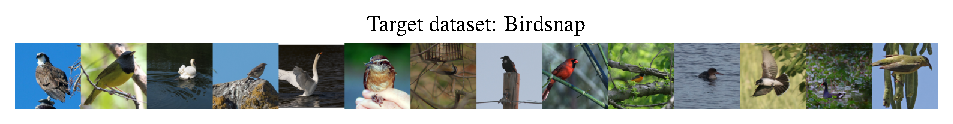
\includegraphics{figures/birdsnap_targets.pdf} \\
    \vspace{-0.8em}
    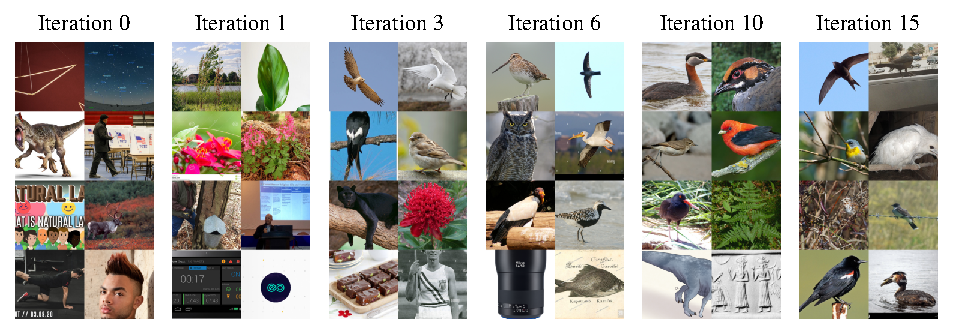
\includegraphics{figures/birdsnap-progression-1146-2col.pdf}
    \caption{\textbf{Progression of downloaded Birdsnap images.} This corresponds to Ours++ without using label set information. }
    \label{fig:birdsnap_progression}
\end{figure*}

\begin{figure*}
    \centering
    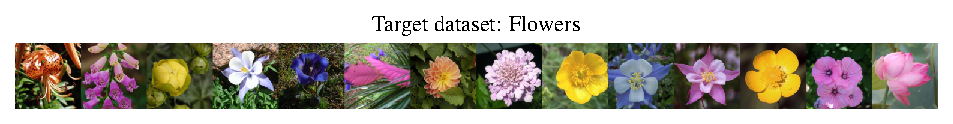
\includegraphics{figures/flowers_targets.pdf} \\
    \vspace{-0.8em}
    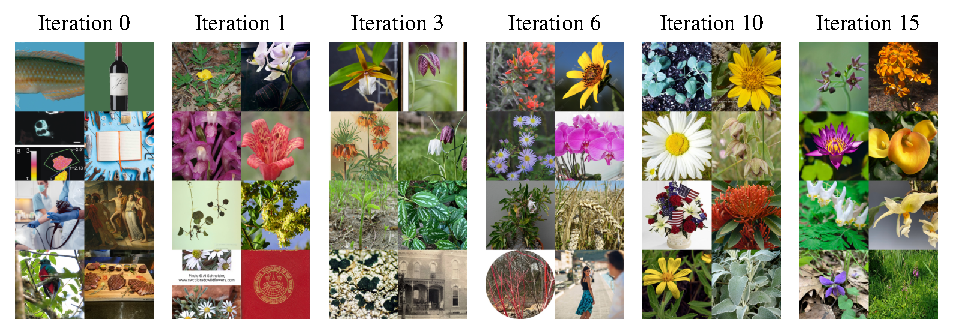
\includegraphics{figures/flowers-progression-1150-2col.pdf}
    \caption{\textbf{Progression of downloaded Flowers images.} This corresponds to Ours++ without using label set information. }
    \label{fig:flowers_progression}
\end{figure*}

\begin{figure*}
    \centering
    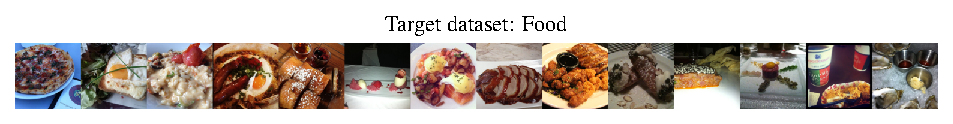
\includegraphics{figures/food_targets.pdf} \\
    \vspace{-0.8em}
    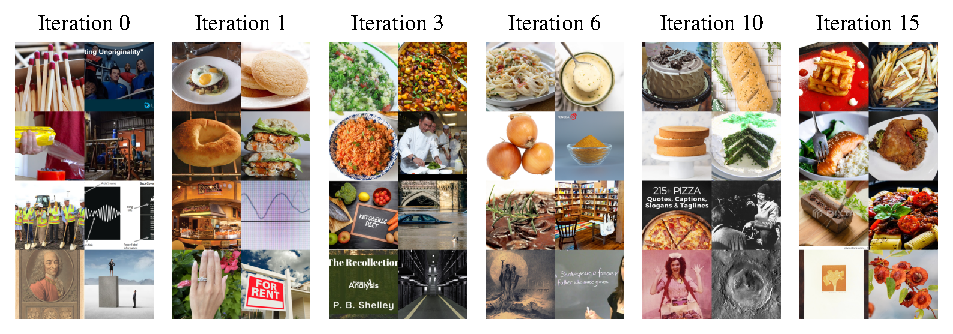
\includegraphics{figures/food-progression-1148-2col.pdf}
    \caption{\textbf{Progression of downloaded Food images.} This corresponds to Ours++ without using label set information. }
    \label{fig:food_progression}
\end{figure*}

\begin{figure*}
    \centering
    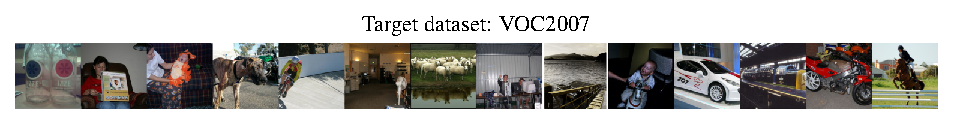
\includegraphics{figures/voc_targets.pdf} \\
    \vspace{-0.8em}
    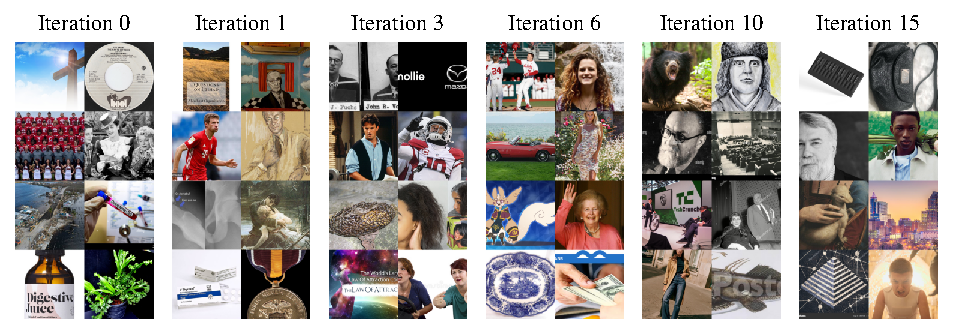
\includegraphics{figures/voc-progression-1156-2col.pdf}
    \caption{\textbf{Progression of downloaded VOC2007 images.} This corresponds to Ours++ without using label set information. }
    \label{fig:voc_progression}
\end{figure*}

% \section{Other experiments:}
% \begin{itemize}
% \item do we need GP or not 
% \item do we need std + mean or not 
% \end{itemize}

%%%%%%%%%%%%%%%%%%%%%%%%%%%%%%%%%%%%%%%%%%%%%%%%%%%%%%%%%%%%%%%%%%%%%%%%%%%%%%%
%%%%%%%%%%%%%%%%%%%%%%%%%%%%%%%%%%%%%%%%%%%%%%%%%%%%%%%%%%%%%%%%%%%%%%%%%%%%%%%

\section{Additional Figures}
\begin{figure}
    \centering
    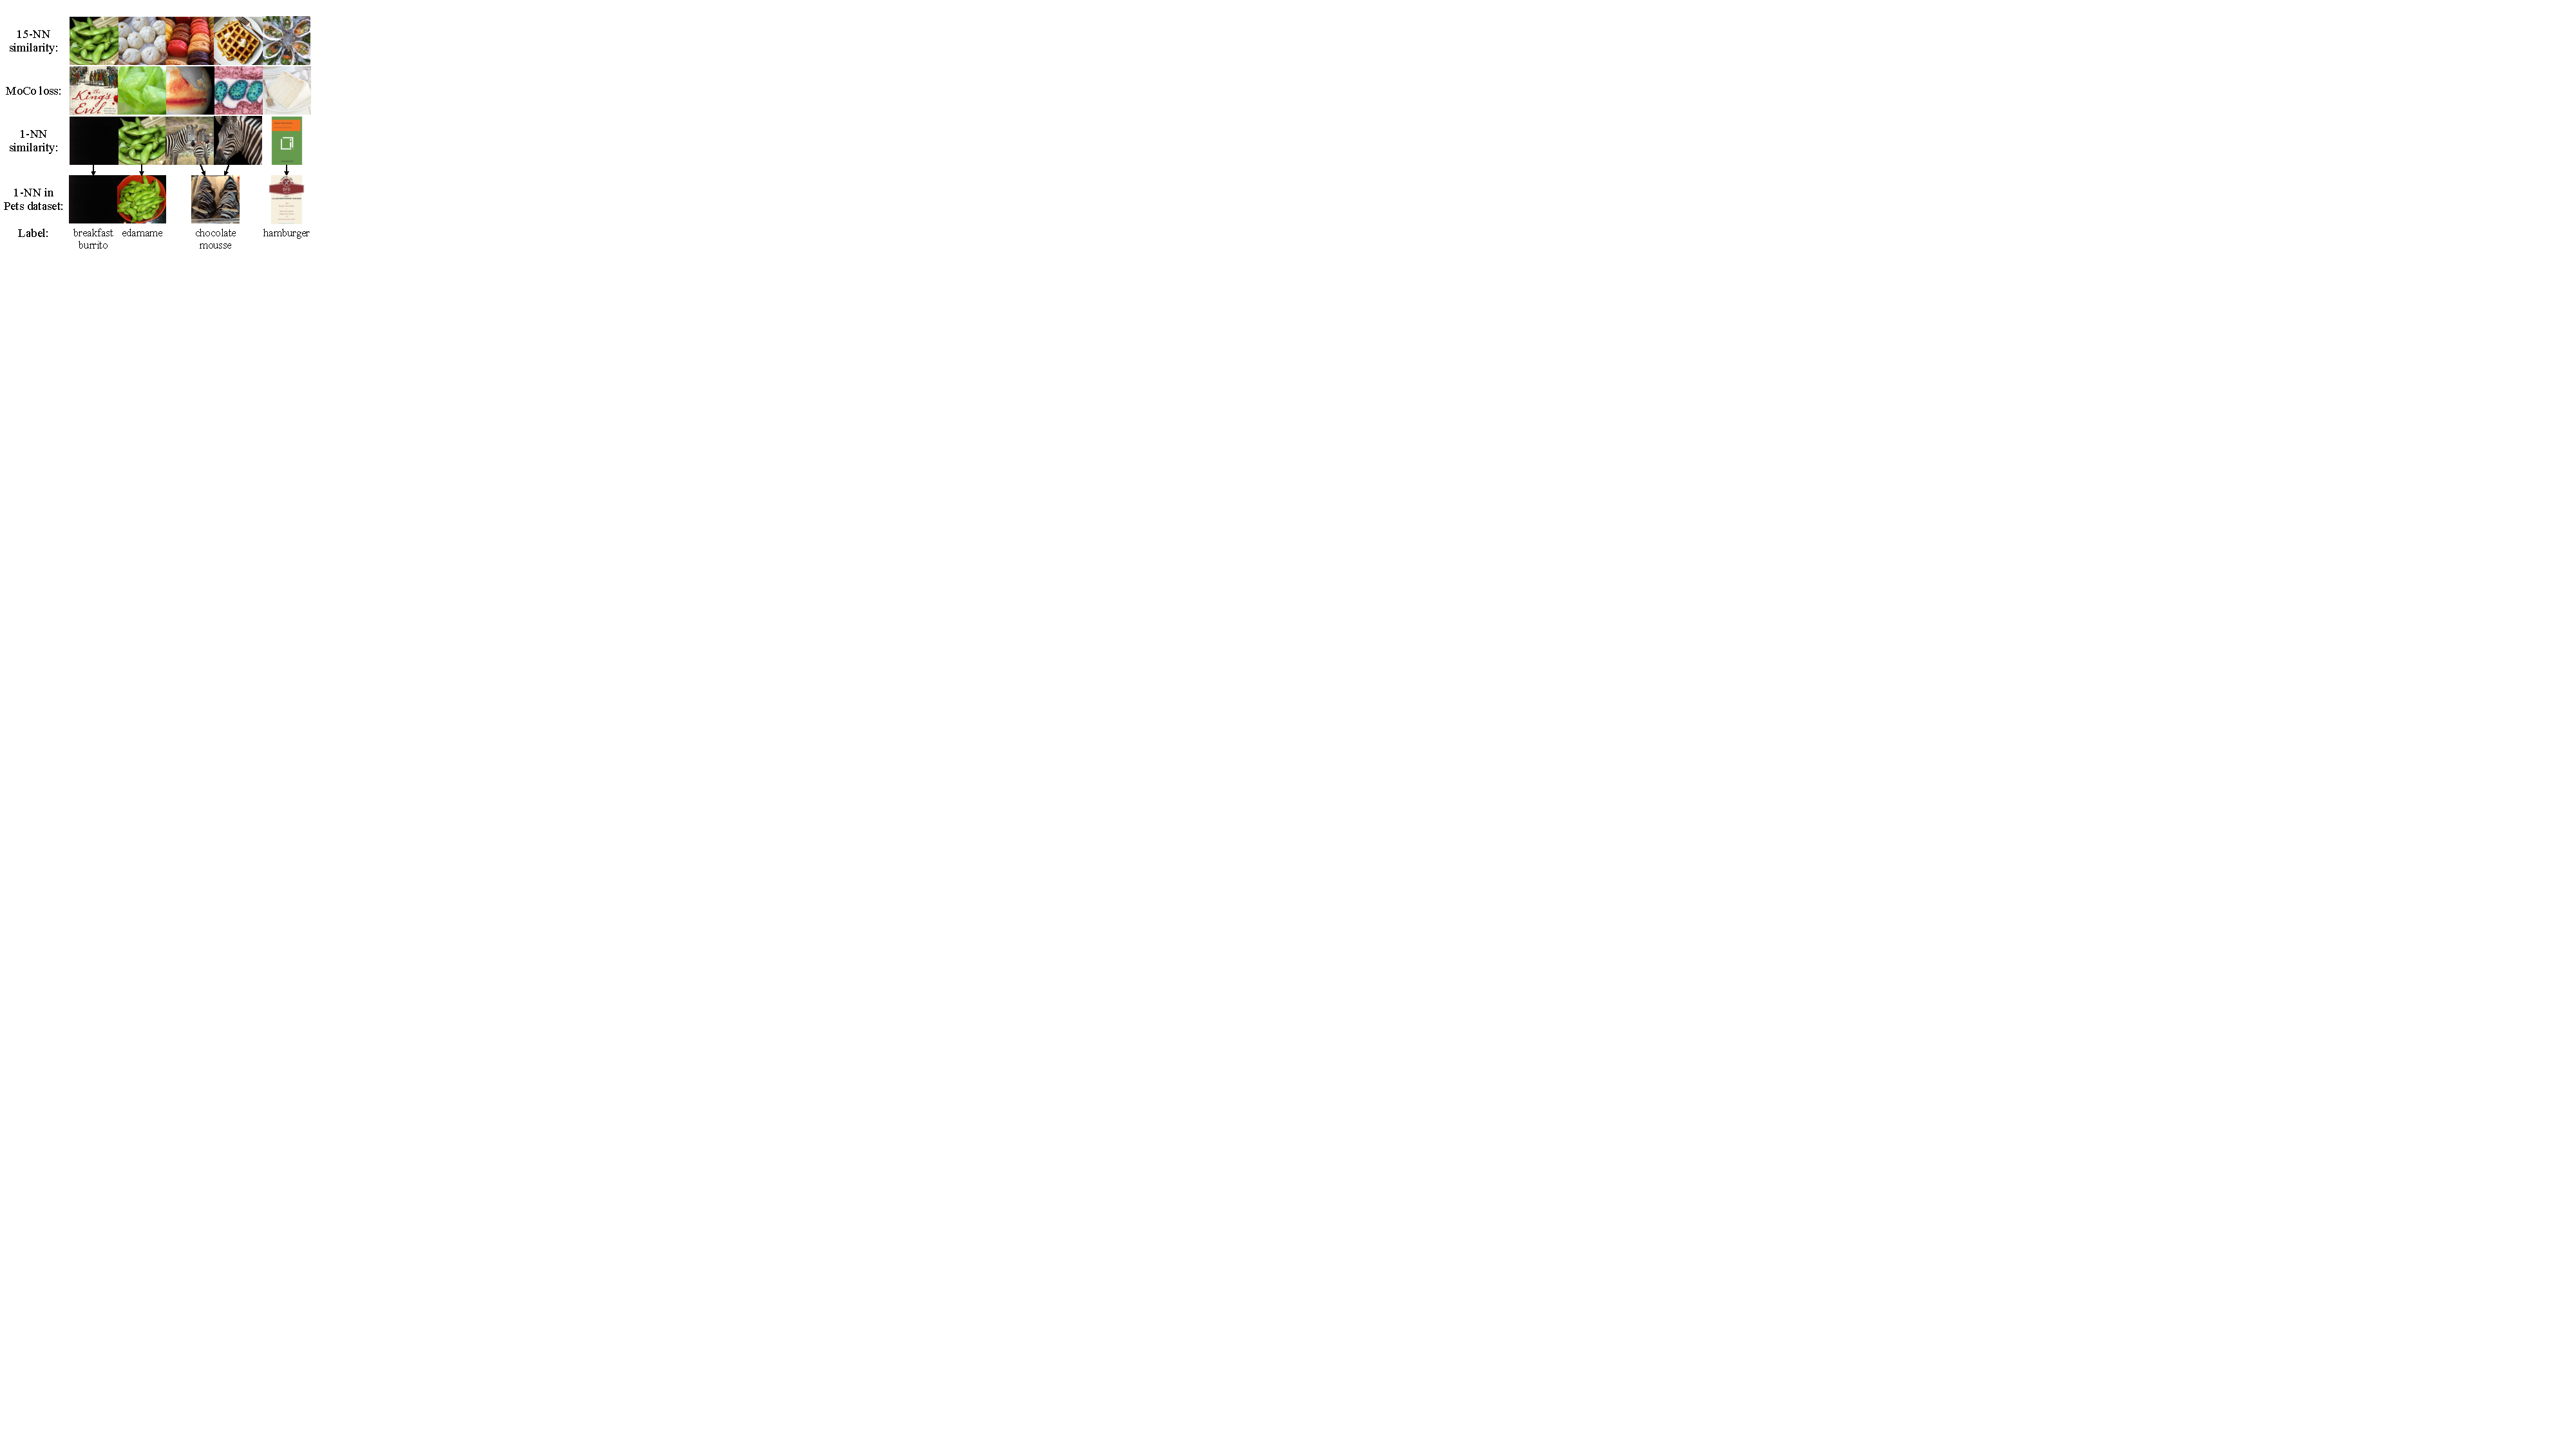
\includegraphics[width=0.5\linewidth]{figures/reward_ranking.pdf}
    % \vspace{-0.25in}
    \caption{\textbf{Top images preferred by different rewards.} We show the top 5 downloaded images ranked by 3 possible image rewards on the Food dataset. 15-NN (ours) prefers a variety of food images, whereas MoCo prefers noisy images out of the training distribution. 1-NN is thrown off by outliers in the Food dataset and thus prefers black images, text, and zebras.}
    \label{fig:reward_ranking}
    % \vspace{-0.06in}
\end{figure}

%%% Local Variables:
%%% coding: utf-8
%%% mode: latex
%%% TeX-engine: xetex
%%% TeX-master: "../thesis"
%%% End: